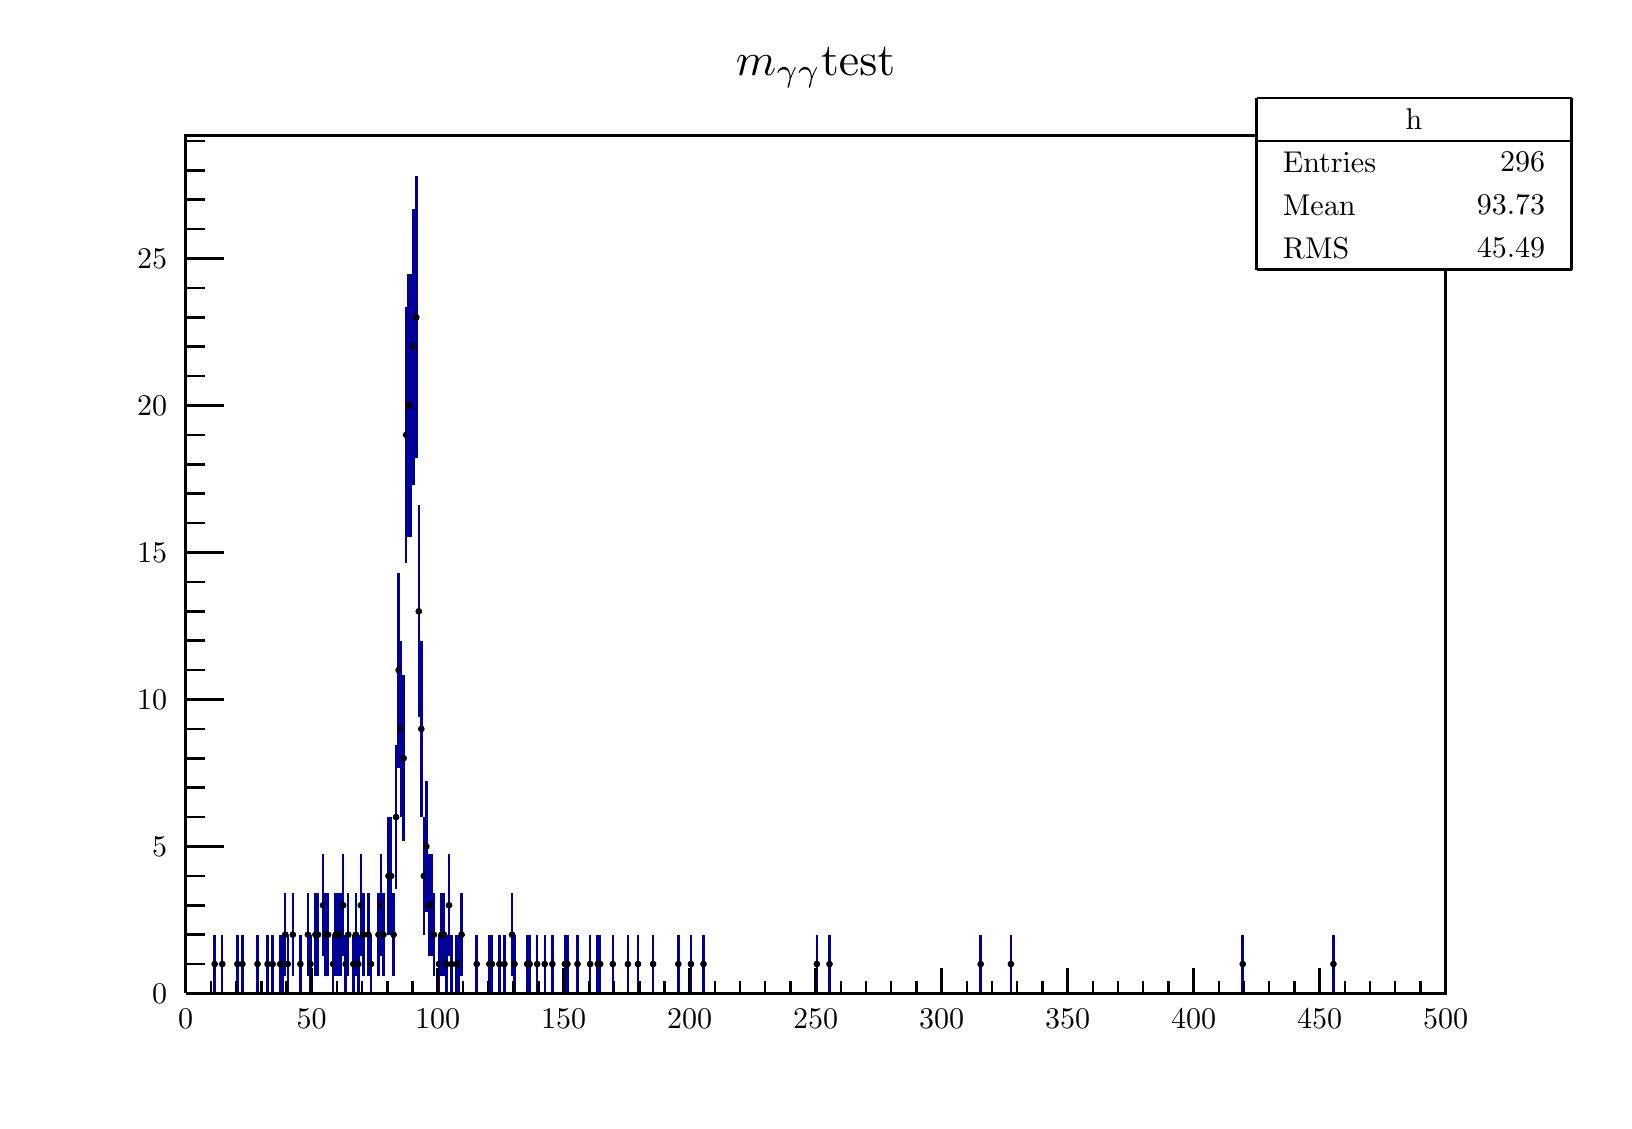
\begin{tikzpicture}
\pgfdeclareplotmark{cross} {
\pgfpathmoveto{\pgfpoint{-0.3\pgfplotmarksize}{\pgfplotmarksize}}
\pgfpathlineto{\pgfpoint{+0.3\pgfplotmarksize}{\pgfplotmarksize}}
\pgfpathlineto{\pgfpoint{+0.3\pgfplotmarksize}{0.3\pgfplotmarksize}}
\pgfpathlineto{\pgfpoint{+1\pgfplotmarksize}{0.3\pgfplotmarksize}}
\pgfpathlineto{\pgfpoint{+1\pgfplotmarksize}{-0.3\pgfplotmarksize}}
\pgfpathlineto{\pgfpoint{+0.3\pgfplotmarksize}{-0.3\pgfplotmarksize}}
\pgfpathlineto{\pgfpoint{+0.3\pgfplotmarksize}{-1.\pgfplotmarksize}}
\pgfpathlineto{\pgfpoint{-0.3\pgfplotmarksize}{-1.\pgfplotmarksize}}
\pgfpathlineto{\pgfpoint{-0.3\pgfplotmarksize}{-0.3\pgfplotmarksize}}
\pgfpathlineto{\pgfpoint{-1.\pgfplotmarksize}{-0.3\pgfplotmarksize}}
\pgfpathlineto{\pgfpoint{-1.\pgfplotmarksize}{0.3\pgfplotmarksize}}
\pgfpathlineto{\pgfpoint{-0.3\pgfplotmarksize}{0.3\pgfplotmarksize}}
\pgfpathclose
\pgfusepathqstroke
}
\pgfdeclareplotmark{cross*} {
\pgfpathmoveto{\pgfpoint{-0.3\pgfplotmarksize}{\pgfplotmarksize}}
\pgfpathlineto{\pgfpoint{+0.3\pgfplotmarksize}{\pgfplotmarksize}}
\pgfpathlineto{\pgfpoint{+0.3\pgfplotmarksize}{0.3\pgfplotmarksize}}
\pgfpathlineto{\pgfpoint{+1\pgfplotmarksize}{0.3\pgfplotmarksize}}
\pgfpathlineto{\pgfpoint{+1\pgfplotmarksize}{-0.3\pgfplotmarksize}}
\pgfpathlineto{\pgfpoint{+0.3\pgfplotmarksize}{-0.3\pgfplotmarksize}}
\pgfpathlineto{\pgfpoint{+0.3\pgfplotmarksize}{-1.\pgfplotmarksize}}
\pgfpathlineto{\pgfpoint{-0.3\pgfplotmarksize}{-1.\pgfplotmarksize}}
\pgfpathlineto{\pgfpoint{-0.3\pgfplotmarksize}{-0.3\pgfplotmarksize}}
\pgfpathlineto{\pgfpoint{-1.\pgfplotmarksize}{-0.3\pgfplotmarksize}}
\pgfpathlineto{\pgfpoint{-1.\pgfplotmarksize}{0.3\pgfplotmarksize}}
\pgfpathlineto{\pgfpoint{-0.3\pgfplotmarksize}{0.3\pgfplotmarksize}}
\pgfpathclose
\pgfusepathqfillstroke
}
\pgfdeclareplotmark{newstar} {
\pgfpathmoveto{\pgfqpoint{0pt}{\pgfplotmarksize}}
\pgfpathlineto{\pgfqpointpolar{44}{0.5\pgfplotmarksize}}
\pgfpathlineto{\pgfqpointpolar{18}{\pgfplotmarksize}}
\pgfpathlineto{\pgfqpointpolar{-20}{0.5\pgfplotmarksize}}
\pgfpathlineto{\pgfqpointpolar{-54}{\pgfplotmarksize}}
\pgfpathlineto{\pgfqpointpolar{-90}{0.5\pgfplotmarksize}}
\pgfpathlineto{\pgfqpointpolar{234}{\pgfplotmarksize}}
\pgfpathlineto{\pgfqpointpolar{198}{0.5\pgfplotmarksize}}
\pgfpathlineto{\pgfqpointpolar{162}{\pgfplotmarksize}}
\pgfpathlineto{\pgfqpointpolar{134}{0.5\pgfplotmarksize}}
\pgfpathclose
\pgfusepathqstroke
}
\pgfdeclareplotmark{newstar*} {
\pgfpathmoveto{\pgfqpoint{0pt}{\pgfplotmarksize}}
\pgfpathlineto{\pgfqpointpolar{44}{0.5\pgfplotmarksize}}
\pgfpathlineto{\pgfqpointpolar{18}{\pgfplotmarksize}}
\pgfpathlineto{\pgfqpointpolar{-20}{0.5\pgfplotmarksize}}
\pgfpathlineto{\pgfqpointpolar{-54}{\pgfplotmarksize}}
\pgfpathlineto{\pgfqpointpolar{-90}{0.5\pgfplotmarksize}}
\pgfpathlineto{\pgfqpointpolar{234}{\pgfplotmarksize}}
\pgfpathlineto{\pgfqpointpolar{198}{0.5\pgfplotmarksize}}
\pgfpathlineto{\pgfqpointpolar{162}{\pgfplotmarksize}}
\pgfpathlineto{\pgfqpointpolar{134}{0.5\pgfplotmarksize}}
\pgfpathclose
\pgfusepathqfillstroke
}
\definecolor{c}{rgb}{1,1,1};
\draw [color=c, fill=c] (0,0) rectangle (20,13.6207);
\draw [color=c, fill=c] (2,1.36207) rectangle (18,12.2586);
\definecolor{c}{rgb}{0,0,0};
\draw [c,line width=0.9] (2,1.36207) -- (2,12.2586) -- (18,12.2586) -- (18,1.36207) -- (2,1.36207);
\definecolor{c}{rgb}{1,1,1};
\draw [color=c, fill=c] (2,1.36207) rectangle (18,12.2586);
\definecolor{c}{rgb}{0,0,0};
\draw [c,line width=0.9] (2,1.36207) -- (2,12.2586) -- (18,12.2586) -- (18,1.36207) -- (2,1.36207);
\definecolor{c}{rgb}{0,0,0.6};
\draw [c,line width=0.9] (2.368,1.36207) -- (2.368,1.73542);
\draw [c,line width=0.9] (2.368,1.73542) -- (2.368,2.10878);
\draw [c,line width=0.9] (2.352,1.73542) -- (2.368,1.73542);
\draw [c,line width=0.9] (2.368,1.73542) -- (2.384,1.73542);
\definecolor{c}{rgb}{0,0,0};
\foreach \P in {(2.368,1.73542)}{\draw[mark options={color=c,fill=c},mark size=2.402402pt,mark=*,mark size=1pt] plot coordinates {\P};}
\definecolor{c}{rgb}{0,0,0.6};
\draw [c,line width=0.9] (2.464,1.36207) -- (2.464,1.73542);
\draw [c,line width=0.9] (2.464,1.73542) -- (2.464,2.10878);
\draw [c,line width=0.9] (2.448,1.73542) -- (2.464,1.73542);
\draw [c,line width=0.9] (2.464,1.73542) -- (2.48,1.73542);
\definecolor{c}{rgb}{0,0,0};
\foreach \P in {(2.464,1.73542)}{\draw[mark options={color=c,fill=c},mark size=2.402402pt,mark=*,mark size=1pt] plot coordinates {\P};}
\definecolor{c}{rgb}{0,0,0.6};
\draw [c,line width=0.9] (2.656,1.36207) -- (2.656,1.73542);
\draw [c,line width=0.9] (2.656,1.73542) -- (2.656,2.10878);
\draw [c,line width=0.9] (2.64,1.73542) -- (2.656,1.73542);
\draw [c,line width=0.9] (2.656,1.73542) -- (2.672,1.73542);
\definecolor{c}{rgb}{0,0,0};
\foreach \P in {(2.656,1.73542)}{\draw[mark options={color=c,fill=c},mark size=2.402402pt,mark=*,mark size=1pt] plot coordinates {\P};}
\definecolor{c}{rgb}{0,0,0.6};
\draw [c,line width=0.9] (2.72,1.36207) -- (2.72,1.73542);
\draw [c,line width=0.9] (2.72,1.73542) -- (2.72,2.10878);
\draw [c,line width=0.9] (2.704,1.73542) -- (2.72,1.73542);
\draw [c,line width=0.9] (2.72,1.73542) -- (2.736,1.73542);
\definecolor{c}{rgb}{0,0,0};
\foreach \P in {(2.72,1.73542)}{\draw[mark options={color=c,fill=c},mark size=2.402402pt,mark=*,mark size=1pt] plot coordinates {\P};}
\definecolor{c}{rgb}{0,0,0.6};
\draw [c,line width=0.9] (2.912,1.36207) -- (2.912,1.73542);
\draw [c,line width=0.9] (2.912,1.73542) -- (2.912,2.10878);
\draw [c,line width=0.9] (2.896,1.73542) -- (2.912,1.73542);
\draw [c,line width=0.9] (2.912,1.73542) -- (2.928,1.73542);
\definecolor{c}{rgb}{0,0,0};
\foreach \P in {(2.912,1.73542)}{\draw[mark options={color=c,fill=c},mark size=2.402402pt,mark=*,mark size=1pt] plot coordinates {\P};}
\definecolor{c}{rgb}{0,0,0.6};
\draw [c,line width=0.9] (3.04,1.36207) -- (3.04,1.73542);
\draw [c,line width=0.9] (3.04,1.73542) -- (3.04,2.10878);
\draw [c,line width=0.9] (3.024,1.73542) -- (3.04,1.73542);
\draw [c,line width=0.9] (3.04,1.73542) -- (3.056,1.73542);
\definecolor{c}{rgb}{0,0,0};
\foreach \P in {(3.04,1.73542)}{\draw[mark options={color=c,fill=c},mark size=2.402402pt,mark=*,mark size=1pt] plot coordinates {\P};}
\definecolor{c}{rgb}{0,0,0.6};
\draw [c,line width=0.9] (3.104,1.36207) -- (3.104,1.73542);
\draw [c,line width=0.9] (3.104,1.73542) -- (3.104,2.10878);
\draw [c,line width=0.9] (3.088,1.73542) -- (3.104,1.73542);
\draw [c,line width=0.9] (3.104,1.73542) -- (3.12,1.73542);
\definecolor{c}{rgb}{0,0,0};
\foreach \P in {(3.104,1.73542)}{\draw[mark options={color=c,fill=c},mark size=2.402402pt,mark=*,mark size=1pt] plot coordinates {\P};}
\definecolor{c}{rgb}{0,0,0.6};
\draw [c,line width=0.9] (3.2,1.36207) -- (3.2,1.73542);
\draw [c,line width=0.9] (3.2,1.73542) -- (3.2,2.10878);
\draw [c,line width=0.9] (3.184,1.73542) -- (3.2,1.73542);
\draw [c,line width=0.9] (3.2,1.73542) -- (3.216,1.73542);
\definecolor{c}{rgb}{0,0,0};
\foreach \P in {(3.2,1.73542)}{\draw[mark options={color=c,fill=c},mark size=2.402402pt,mark=*,mark size=1pt] plot coordinates {\P};}
\definecolor{c}{rgb}{0,0,0.6};
\draw [c,line width=0.9] (3.232,1.36207) -- (3.232,1.73542);
\draw [c,line width=0.9] (3.232,1.73542) -- (3.232,2.10878);
\draw [c,line width=0.9] (3.216,1.73542) -- (3.232,1.73542);
\draw [c,line width=0.9] (3.232,1.73542) -- (3.248,1.73542);
\definecolor{c}{rgb}{0,0,0};
\foreach \P in {(3.232,1.73542)}{\draw[mark options={color=c,fill=c},mark size=2.402402pt,mark=*,mark size=1pt] plot coordinates {\P};}
\definecolor{c}{rgb}{0,0,0.6};
\draw [c,line width=0.9] (3.264,1.58077) -- (3.264,2.10878);
\draw [c,line width=0.9] (3.264,2.10878) -- (3.264,2.63678);
\draw [c,line width=0.9] (3.248,2.10878) -- (3.264,2.10878);
\draw [c,line width=0.9] (3.264,2.10878) -- (3.28,2.10878);
\definecolor{c}{rgb}{0,0,0};
\foreach \P in {(3.264,2.10878)}{\draw[mark options={color=c,fill=c},mark size=2.402402pt,mark=*,mark size=1pt] plot coordinates {\P};}
\definecolor{c}{rgb}{0,0,0.6};
\draw [c,line width=0.9] (3.296,1.36207) -- (3.296,1.73542);
\draw [c,line width=0.9] (3.296,1.73542) -- (3.296,2.10878);
\draw [c,line width=0.9] (3.28,1.73542) -- (3.296,1.73542);
\draw [c,line width=0.9] (3.296,1.73542) -- (3.312,1.73542);
\definecolor{c}{rgb}{0,0,0};
\foreach \P in {(3.296,1.73542)}{\draw[mark options={color=c,fill=c},mark size=2.402402pt,mark=*,mark size=1pt] plot coordinates {\P};}
\definecolor{c}{rgb}{0,0,0.6};
\draw [c,line width=0.9] (3.36,1.58077) -- (3.36,2.10878);
\draw [c,line width=0.9] (3.36,2.10878) -- (3.36,2.63678);
\draw [c,line width=0.9] (3.344,2.10878) -- (3.36,2.10878);
\draw [c,line width=0.9] (3.36,2.10878) -- (3.376,2.10878);
\definecolor{c}{rgb}{0,0,0};
\foreach \P in {(3.36,2.10878)}{\draw[mark options={color=c,fill=c},mark size=2.402402pt,mark=*,mark size=1pt] plot coordinates {\P};}
\definecolor{c}{rgb}{0,0,0.6};
\draw [c,line width=0.9] (3.456,1.36207) -- (3.456,1.73542);
\draw [c,line width=0.9] (3.456,1.73542) -- (3.456,2.10878);
\draw [c,line width=0.9] (3.44,1.73542) -- (3.456,1.73542);
\draw [c,line width=0.9] (3.456,1.73542) -- (3.472,1.73542);
\definecolor{c}{rgb}{0,0,0};
\foreach \P in {(3.456,1.73542)}{\draw[mark options={color=c,fill=c},mark size=2.402402pt,mark=*,mark size=1pt] plot coordinates {\P};}
\definecolor{c}{rgb}{0,0,0.6};
\draw [c,line width=0.9] (3.552,1.58077) -- (3.552,2.10878);
\draw [c,line width=0.9] (3.552,2.10878) -- (3.552,2.63678);
\draw [c,line width=0.9] (3.536,2.10878) -- (3.552,2.10878);
\draw [c,line width=0.9] (3.552,2.10878) -- (3.568,2.10878);
\definecolor{c}{rgb}{0,0,0};
\foreach \P in {(3.552,2.10878)}{\draw[mark options={color=c,fill=c},mark size=2.402402pt,mark=*,mark size=1pt] plot coordinates {\P};}
\definecolor{c}{rgb}{0,0,0.6};
\draw [c,line width=0.9] (3.584,1.36207) -- (3.584,1.73542);
\draw [c,line width=0.9] (3.584,1.73542) -- (3.584,2.10878);
\draw [c,line width=0.9] (3.568,1.73542) -- (3.584,1.73542);
\draw [c,line width=0.9] (3.584,1.73542) -- (3.6,1.73542);
\definecolor{c}{rgb}{0,0,0};
\foreach \P in {(3.584,1.73542)}{\draw[mark options={color=c,fill=c},mark size=2.402402pt,mark=*,mark size=1pt] plot coordinates {\P};}
\definecolor{c}{rgb}{0,0,0.6};
\draw [c,line width=0.9] (3.648,1.58077) -- (3.648,2.10878);
\draw [c,line width=0.9] (3.648,2.10878) -- (3.648,2.63678);
\draw [c,line width=0.9] (3.632,2.10878) -- (3.648,2.10878);
\draw [c,line width=0.9] (3.648,2.10878) -- (3.664,2.10878);
\definecolor{c}{rgb}{0,0,0};
\foreach \P in {(3.648,2.10878)}{\draw[mark options={color=c,fill=c},mark size=2.402402pt,mark=*,mark size=1pt] plot coordinates {\P};}
\definecolor{c}{rgb}{0,0,0.6};
\draw [c,line width=0.9] (3.68,1.58077) -- (3.68,2.10878);
\draw [c,line width=0.9] (3.68,2.10878) -- (3.68,2.63678);
\draw [c,line width=0.9] (3.664,2.10878) -- (3.68,2.10878);
\draw [c,line width=0.9] (3.68,2.10878) -- (3.696,2.10878);
\definecolor{c}{rgb}{0,0,0};
\foreach \P in {(3.68,2.10878)}{\draw[mark options={color=c,fill=c},mark size=2.402402pt,mark=*,mark size=1pt] plot coordinates {\P};}
\definecolor{c}{rgb}{0,0,0.6};
\draw [c,line width=0.9] (3.744,1.83546) -- (3.744,2.48213);
\draw [c,line width=0.9] (3.744,2.48213) -- (3.744,3.1288);
\draw [c,line width=0.9] (3.728,2.48213) -- (3.744,2.48213);
\draw [c,line width=0.9] (3.744,2.48213) -- (3.76,2.48213);
\definecolor{c}{rgb}{0,0,0};
\foreach \P in {(3.744,2.48213)}{\draw[mark options={color=c,fill=c},mark size=2.402402pt,mark=*,mark size=1pt] plot coordinates {\P};}
\definecolor{c}{rgb}{0,0,0.6};
\draw [c,line width=0.9] (3.776,1.58077) -- (3.776,2.10878);
\draw [c,line width=0.9] (3.776,2.10878) -- (3.776,2.63678);
\draw [c,line width=0.9] (3.76,2.10878) -- (3.776,2.10878);
\draw [c,line width=0.9] (3.776,2.10878) -- (3.792,2.10878);
\definecolor{c}{rgb}{0,0,0};
\foreach \P in {(3.776,2.10878)}{\draw[mark options={color=c,fill=c},mark size=2.402402pt,mark=*,mark size=1pt] plot coordinates {\P};}
\definecolor{c}{rgb}{0,0,0.6};
\draw [c,line width=0.9] (3.808,1.58077) -- (3.808,2.10878);
\draw [c,line width=0.9] (3.808,2.10878) -- (3.808,2.63678);
\draw [c,line width=0.9] (3.792,2.10878) -- (3.808,2.10878);
\draw [c,line width=0.9] (3.808,2.10878) -- (3.824,2.10878);
\definecolor{c}{rgb}{0,0,0};
\foreach \P in {(3.808,2.10878)}{\draw[mark options={color=c,fill=c},mark size=2.402402pt,mark=*,mark size=1pt] plot coordinates {\P};}
\definecolor{c}{rgb}{0,0,0.6};
\draw [c,line width=0.9] (3.872,1.36207) -- (3.872,1.73542);
\draw [c,line width=0.9] (3.872,1.73542) -- (3.872,2.10878);
\draw [c,line width=0.9] (3.856,1.73542) -- (3.872,1.73542);
\draw [c,line width=0.9] (3.872,1.73542) -- (3.888,1.73542);
\definecolor{c}{rgb}{0,0,0};
\foreach \P in {(3.872,1.73542)}{\draw[mark options={color=c,fill=c},mark size=2.402402pt,mark=*,mark size=1pt] plot coordinates {\P};}
\definecolor{c}{rgb}{0,0,0.6};
\draw [c,line width=0.9] (3.904,1.58077) -- (3.904,2.10878);
\draw [c,line width=0.9] (3.904,2.10878) -- (3.904,2.63678);
\draw [c,line width=0.9] (3.888,2.10878) -- (3.904,2.10878);
\draw [c,line width=0.9] (3.904,2.10878) -- (3.92,2.10878);
\definecolor{c}{rgb}{0,0,0};
\foreach \P in {(3.904,2.10878)}{\draw[mark options={color=c,fill=c},mark size=2.402402pt,mark=*,mark size=1pt] plot coordinates {\P};}
\definecolor{c}{rgb}{0,0,0.6};
\draw [c,line width=0.9] (3.936,1.58077) -- (3.936,2.10878);
\draw [c,line width=0.9] (3.936,2.10878) -- (3.936,2.63678);
\draw [c,line width=0.9] (3.92,2.10878) -- (3.936,2.10878);
\draw [c,line width=0.9] (3.936,2.10878) -- (3.952,2.10878);
\definecolor{c}{rgb}{0,0,0};
\foreach \P in {(3.936,2.10878)}{\draw[mark options={color=c,fill=c},mark size=2.402402pt,mark=*,mark size=1pt] plot coordinates {\P};}
\definecolor{c}{rgb}{0,0,0.6};
\draw [c,line width=0.9] (3.968,1.58077) -- (3.968,2.10878);
\draw [c,line width=0.9] (3.968,2.10878) -- (3.968,2.63678);
\draw [c,line width=0.9] (3.952,2.10878) -- (3.968,2.10878);
\draw [c,line width=0.9] (3.968,2.10878) -- (3.984,2.10878);
\definecolor{c}{rgb}{0,0,0};
\foreach \P in {(3.968,2.10878)}{\draw[mark options={color=c,fill=c},mark size=2.402402pt,mark=*,mark size=1pt] plot coordinates {\P};}
\definecolor{c}{rgb}{0,0,0.6};
\draw [c,line width=0.9] (4,1.83546) -- (4,2.48213);
\draw [c,line width=0.9] (4,2.48213) -- (4,3.1288);
\draw [c,line width=0.9] (3.984,2.48213) -- (4,2.48213);
\draw [c,line width=0.9] (4,2.48213) -- (4.016,2.48213);
\definecolor{c}{rgb}{0,0,0};
\foreach \P in {(4,2.48213)}{\draw[mark options={color=c,fill=c},mark size=2.402402pt,mark=*,mark size=1pt] plot coordinates {\P};}
\definecolor{c}{rgb}{0,0,0.6};
\draw [c,line width=0.9] (4.032,1.36207) -- (4.032,1.73542);
\draw [c,line width=0.9] (4.032,1.73542) -- (4.032,2.10878);
\draw [c,line width=0.9] (4.016,1.73542) -- (4.032,1.73542);
\draw [c,line width=0.9] (4.032,1.73542) -- (4.048,1.73542);
\definecolor{c}{rgb}{0,0,0};
\foreach \P in {(4.032,1.73542)}{\draw[mark options={color=c,fill=c},mark size=2.402402pt,mark=*,mark size=1pt] plot coordinates {\P};}
\definecolor{c}{rgb}{0,0,0.6};
\draw [c,line width=0.9] (4.064,1.58077) -- (4.064,2.10878);
\draw [c,line width=0.9] (4.064,2.10878) -- (4.064,2.63678);
\draw [c,line width=0.9] (4.048,2.10878) -- (4.064,2.10878);
\draw [c,line width=0.9] (4.064,2.10878) -- (4.08,2.10878);
\definecolor{c}{rgb}{0,0,0};
\foreach \P in {(4.064,2.10878)}{\draw[mark options={color=c,fill=c},mark size=2.402402pt,mark=*,mark size=1pt] plot coordinates {\P};}
\definecolor{c}{rgb}{0,0,0.6};
\draw [c,line width=0.9] (4.128,1.36207) -- (4.128,1.73542);
\draw [c,line width=0.9] (4.128,1.73542) -- (4.128,2.10878);
\draw [c,line width=0.9] (4.112,1.73542) -- (4.128,1.73542);
\draw [c,line width=0.9] (4.128,1.73542) -- (4.144,1.73542);
\definecolor{c}{rgb}{0,0,0};
\foreach \P in {(4.128,1.73542)}{\draw[mark options={color=c,fill=c},mark size=2.402402pt,mark=*,mark size=1pt] plot coordinates {\P};}
\definecolor{c}{rgb}{0,0,0.6};
\draw [c,line width=0.9] (4.16,1.58077) -- (4.16,2.10878);
\draw [c,line width=0.9] (4.16,2.10878) -- (4.16,2.63678);
\draw [c,line width=0.9] (4.144,2.10878) -- (4.16,2.10878);
\draw [c,line width=0.9] (4.16,2.10878) -- (4.176,2.10878);
\definecolor{c}{rgb}{0,0,0};
\foreach \P in {(4.16,2.10878)}{\draw[mark options={color=c,fill=c},mark size=2.402402pt,mark=*,mark size=1pt] plot coordinates {\P};}
\definecolor{c}{rgb}{0,0,0.6};
\draw [c,line width=0.9] (4.192,1.36207) -- (4.192,1.73542);
\draw [c,line width=0.9] (4.192,1.73542) -- (4.192,2.10878);
\draw [c,line width=0.9] (4.176,1.73542) -- (4.192,1.73542);
\draw [c,line width=0.9] (4.192,1.73542) -- (4.208,1.73542);
\definecolor{c}{rgb}{0,0,0};
\foreach \P in {(4.192,1.73542)}{\draw[mark options={color=c,fill=c},mark size=2.402402pt,mark=*,mark size=1pt] plot coordinates {\P};}
\definecolor{c}{rgb}{0,0,0.6};
\draw [c,line width=0.9] (4.224,1.83546) -- (4.224,2.48213);
\draw [c,line width=0.9] (4.224,2.48213) -- (4.224,3.1288);
\draw [c,line width=0.9] (4.208,2.48213) -- (4.224,2.48213);
\draw [c,line width=0.9] (4.224,2.48213) -- (4.24,2.48213);
\definecolor{c}{rgb}{0,0,0};
\foreach \P in {(4.224,2.48213)}{\draw[mark options={color=c,fill=c},mark size=2.402402pt,mark=*,mark size=1pt] plot coordinates {\P};}
\definecolor{c}{rgb}{0,0,0.6};
\draw [c,line width=0.9] (4.256,1.58077) -- (4.256,2.10878);
\draw [c,line width=0.9] (4.256,2.10878) -- (4.256,2.63678);
\draw [c,line width=0.9] (4.24,2.10878) -- (4.256,2.10878);
\draw [c,line width=0.9] (4.256,2.10878) -- (4.272,2.10878);
\definecolor{c}{rgb}{0,0,0};
\foreach \P in {(4.256,2.10878)}{\draw[mark options={color=c,fill=c},mark size=2.402402pt,mark=*,mark size=1pt] plot coordinates {\P};}
\definecolor{c}{rgb}{0,0,0.6};
\draw [c,line width=0.9] (4.32,1.58077) -- (4.32,2.10878);
\draw [c,line width=0.9] (4.32,2.10878) -- (4.32,2.63678);
\draw [c,line width=0.9] (4.304,2.10878) -- (4.32,2.10878);
\draw [c,line width=0.9] (4.32,2.10878) -- (4.336,2.10878);
\definecolor{c}{rgb}{0,0,0};
\foreach \P in {(4.32,2.10878)}{\draw[mark options={color=c,fill=c},mark size=2.402402pt,mark=*,mark size=1pt] plot coordinates {\P};}
\definecolor{c}{rgb}{0,0,0.6};
\draw [c,line width=0.9] (4.352,1.36207) -- (4.352,1.73542);
\draw [c,line width=0.9] (4.352,1.73542) -- (4.352,2.10878);
\draw [c,line width=0.9] (4.336,1.73542) -- (4.352,1.73542);
\draw [c,line width=0.9] (4.352,1.73542) -- (4.368,1.73542);
\definecolor{c}{rgb}{0,0,0};
\foreach \P in {(4.352,1.73542)}{\draw[mark options={color=c,fill=c},mark size=2.402402pt,mark=*,mark size=1pt] plot coordinates {\P};}
\definecolor{c}{rgb}{0,0,0.6};
\draw [c,line width=0.9] (4.448,1.58077) -- (4.448,2.10878);
\draw [c,line width=0.9] (4.448,2.10878) -- (4.448,2.63678);
\draw [c,line width=0.9] (4.432,2.10878) -- (4.448,2.10878);
\draw [c,line width=0.9] (4.448,2.10878) -- (4.464,2.10878);
\definecolor{c}{rgb}{0,0,0};
\foreach \P in {(4.448,2.10878)}{\draw[mark options={color=c,fill=c},mark size=2.402402pt,mark=*,mark size=1pt] plot coordinates {\P};}
\definecolor{c}{rgb}{0,0,0.6};
\draw [c,line width=0.9] (4.48,1.83546) -- (4.48,2.48213);
\draw [c,line width=0.9] (4.48,2.48213) -- (4.48,3.1288);
\draw [c,line width=0.9] (4.464,2.48213) -- (4.48,2.48213);
\draw [c,line width=0.9] (4.48,2.48213) -- (4.496,2.48213);
\definecolor{c}{rgb}{0,0,0};
\foreach \P in {(4.48,2.48213)}{\draw[mark options={color=c,fill=c},mark size=2.402402pt,mark=*,mark size=1pt] plot coordinates {\P};}
\definecolor{c}{rgb}{0,0,0.6};
\draw [c,line width=0.9] (4.512,1.58077) -- (4.512,2.10878);
\draw [c,line width=0.9] (4.512,2.10878) -- (4.512,2.63678);
\draw [c,line width=0.9] (4.496,2.10878) -- (4.512,2.10878);
\draw [c,line width=0.9] (4.512,2.10878) -- (4.528,2.10878);
\definecolor{c}{rgb}{0,0,0};
\foreach \P in {(4.512,2.10878)}{\draw[mark options={color=c,fill=c},mark size=2.402402pt,mark=*,mark size=1pt] plot coordinates {\P};}
\definecolor{c}{rgb}{0,0,0.6};
\draw [c,line width=0.9] (4.576,2.10878) -- (4.576,2.85548);
\draw [c,line width=0.9] (4.576,2.85548) -- (4.576,3.60219);
\draw [c,line width=0.9] (4.56,2.85548) -- (4.576,2.85548);
\draw [c,line width=0.9] (4.576,2.85548) -- (4.592,2.85548);
\definecolor{c}{rgb}{0,0,0};
\foreach \P in {(4.576,2.85548)}{\draw[mark options={color=c,fill=c},mark size=2.402402pt,mark=*,mark size=1pt] plot coordinates {\P};}
\definecolor{c}{rgb}{0,0,0.6};
\draw [c,line width=0.9] (4.608,2.10878) -- (4.608,2.85548);
\draw [c,line width=0.9] (4.608,2.85548) -- (4.608,3.60219);
\draw [c,line width=0.9] (4.592,2.85548) -- (4.608,2.85548);
\draw [c,line width=0.9] (4.608,2.85548) -- (4.624,2.85548);
\definecolor{c}{rgb}{0,0,0};
\foreach \P in {(4.608,2.85548)}{\draw[mark options={color=c,fill=c},mark size=2.402402pt,mark=*,mark size=1pt] plot coordinates {\P};}
\definecolor{c}{rgb}{0,0,0.6};
\draw [c,line width=0.9] (4.64,1.58077) -- (4.64,2.10878);
\draw [c,line width=0.9] (4.64,2.10878) -- (4.64,2.63678);
\draw [c,line width=0.9] (4.624,2.10878) -- (4.64,2.10878);
\draw [c,line width=0.9] (4.64,2.10878) -- (4.656,2.10878);
\definecolor{c}{rgb}{0,0,0};
\foreach \P in {(4.64,2.10878)}{\draw[mark options={color=c,fill=c},mark size=2.402402pt,mark=*,mark size=1pt] plot coordinates {\P};}
\definecolor{c}{rgb}{0,0,0.6};
\draw [c,line width=0.9] (4.672,2.68766) -- (4.672,3.60219);
\draw [c,line width=0.9] (4.672,3.60219) -- (4.672,4.51671);
\draw [c,line width=0.9] (4.656,3.60219) -- (4.672,3.60219);
\draw [c,line width=0.9] (4.672,3.60219) -- (4.688,3.60219);
\definecolor{c}{rgb}{0,0,0};
\foreach \P in {(4.672,3.60219)}{\draw[mark options={color=c,fill=c},mark size=2.402402pt,mark=*,mark size=1pt] plot coordinates {\P};}
\definecolor{c}{rgb}{0,0,0.6};
\draw [c,line width=0.9] (4.704,4.23068) -- (4.704,5.46896);
\draw [c,line width=0.9] (4.704,5.46896) -- (4.704,6.70723);
\draw [c,line width=0.9] (4.688,5.46896) -- (4.704,5.46896);
\draw [c,line width=0.9] (4.704,5.46896) -- (4.72,5.46896);
\definecolor{c}{rgb}{0,0,0};
\foreach \P in {(4.704,5.46896)}{\draw[mark options={color=c,fill=c},mark size=2.402402pt,mark=*,mark size=1pt] plot coordinates {\P};}
\definecolor{c}{rgb}{0,0,0.6};
\draw [c,line width=0.9] (4.736,3.60219) -- (4.736,4.72225);
\draw [c,line width=0.9] (4.736,4.72225) -- (4.736,5.84231);
\draw [c,line width=0.9] (4.72,4.72225) -- (4.736,4.72225);
\draw [c,line width=0.9] (4.736,4.72225) -- (4.752,4.72225);
\definecolor{c}{rgb}{0,0,0};
\foreach \P in {(4.736,4.72225)}{\draw[mark options={color=c,fill=c},mark size=2.402402pt,mark=*,mark size=1pt] plot coordinates {\P};}
\definecolor{c}{rgb}{0,0,0.6};
\draw [c,line width=0.9] (4.768,3.29289) -- (4.768,4.3489);
\draw [c,line width=0.9] (4.768,4.3489) -- (4.768,5.4049);
\draw [c,line width=0.9] (4.752,4.3489) -- (4.768,4.3489);
\draw [c,line width=0.9] (4.768,4.3489) -- (4.784,4.3489);
\definecolor{c}{rgb}{0,0,0};
\foreach \P in {(4.768,4.3489)}{\draw[mark options={color=c,fill=c},mark size=2.402402pt,mark=*,mark size=1pt] plot coordinates {\P};}
\definecolor{c}{rgb}{0,0,0.6};
\draw [c,line width=0.9] (4.8,6.82837) -- (4.8,8.45578);
\draw [c,line width=0.9] (4.8,8.45578) -- (4.8,10.0832);
\draw [c,line width=0.9] (4.784,8.45578) -- (4.8,8.45578);
\draw [c,line width=0.9] (4.8,8.45578) -- (4.816,8.45578);
\definecolor{c}{rgb}{0,0,0};
\foreach \P in {(4.8,8.45578)}{\draw[mark options={color=c,fill=c},mark size=2.402402pt,mark=*,mark size=1pt] plot coordinates {\P};}
\definecolor{c}{rgb}{0,0,0.6};
\draw [c,line width=0.9] (4.832,7.15945) -- (4.832,8.82914);
\draw [c,line width=0.9] (4.832,8.82914) -- (4.832,10.4988);
\draw [c,line width=0.9] (4.816,8.82914) -- (4.832,8.82914);
\draw [c,line width=0.9] (4.832,8.82914) -- (4.848,8.82914);
\definecolor{c}{rgb}{0,0,0};
\foreach \P in {(4.832,8.82914)}{\draw[mark options={color=c,fill=c},mark size=2.402402pt,mark=*,mark size=1pt] plot coordinates {\P};}
\definecolor{c}{rgb}{0,0,0.6};
\draw [c,line width=0.9] (4.864,7.15945) -- (4.864,8.82914);
\draw [c,line width=0.9] (4.864,8.82914) -- (4.864,10.4988);
\draw [c,line width=0.9] (4.848,8.82914) -- (4.864,8.82914);
\draw [c,line width=0.9] (4.864,8.82914) -- (4.88,8.82914);
\definecolor{c}{rgb}{0,0,0};
\foreach \P in {(4.864,8.82914)}{\draw[mark options={color=c,fill=c},mark size=2.402402pt,mark=*,mark size=1pt] plot coordinates {\P};}
\definecolor{c}{rgb}{0,0,0.6};
\draw [c,line width=0.9] (4.896,7.82466) -- (4.896,9.57584);
\draw [c,line width=0.9] (4.896,9.57584) -- (4.896,11.327);
\draw [c,line width=0.9] (4.88,9.57584) -- (4.896,9.57584);
\draw [c,line width=0.9] (4.896,9.57584) -- (4.912,9.57584);
\definecolor{c}{rgb}{0,0,0};
\foreach \P in {(4.896,9.57584)}{\draw[mark options={color=c,fill=c},mark size=2.402402pt,mark=*,mark size=1pt] plot coordinates {\P};}
\definecolor{c}{rgb}{0,0,0.6};
\draw [c,line width=0.9] (4.928,8.15866) -- (4.928,9.9492);
\draw [c,line width=0.9] (4.928,9.9492) -- (4.928,11.7397);
\draw [c,line width=0.9] (4.912,9.9492) -- (4.928,9.9492);
\draw [c,line width=0.9] (4.928,9.9492) -- (4.944,9.9492);
\definecolor{c}{rgb}{0,0,0};
\foreach \P in {(4.928,9.9492)}{\draw[mark options={color=c,fill=c},mark size=2.402402pt,mark=*,mark size=1pt] plot coordinates {\P};}
\definecolor{c}{rgb}{0,0,0.6};
\draw [c,line width=0.9] (4.96,4.86952) -- (4.96,6.21566);
\draw [c,line width=0.9] (4.96,6.21566) -- (4.96,7.56181);
\draw [c,line width=0.9] (4.944,6.21566) -- (4.96,6.21566);
\draw [c,line width=0.9] (4.96,6.21566) -- (4.976,6.21566);
\definecolor{c}{rgb}{0,0,0};
\foreach \P in {(4.96,6.21566)}{\draw[mark options={color=c,fill=c},mark size=2.402402pt,mark=*,mark size=1pt] plot coordinates {\P};}
\definecolor{c}{rgb}{0,0,0.6};
\draw [c,line width=0.9] (4.992,3.60219) -- (4.992,4.72225);
\draw [c,line width=0.9] (4.992,4.72225) -- (4.992,5.84231);
\draw [c,line width=0.9] (4.976,4.72225) -- (4.992,4.72225);
\draw [c,line width=0.9] (4.992,4.72225) -- (5.008,4.72225);
\definecolor{c}{rgb}{0,0,0};
\foreach \P in {(4.992,4.72225)}{\draw[mark options={color=c,fill=c},mark size=2.402402pt,mark=*,mark size=1pt] plot coordinates {\P};}
\definecolor{c}{rgb}{0,0,0.6};
\draw [c,line width=0.9] (5.024,2.10878) -- (5.024,2.85548);
\draw [c,line width=0.9] (5.024,2.85548) -- (5.024,3.60219);
\draw [c,line width=0.9] (5.008,2.85548) -- (5.024,2.85548);
\draw [c,line width=0.9] (5.024,2.85548) -- (5.04,2.85548);
\definecolor{c}{rgb}{0,0,0};
\foreach \P in {(5.024,2.85548)}{\draw[mark options={color=c,fill=c},mark size=2.402402pt,mark=*,mark size=1pt] plot coordinates {\P};}
\definecolor{c}{rgb}{0,0,0.6};
\draw [c,line width=0.9] (5.056,2.39399) -- (5.056,3.22884);
\draw [c,line width=0.9] (5.056,3.22884) -- (5.056,4.06368);
\draw [c,line width=0.9] (5.04,3.22884) -- (5.056,3.22884);
\draw [c,line width=0.9] (5.056,3.22884) -- (5.072,3.22884);
\definecolor{c}{rgb}{0,0,0};
\foreach \P in {(5.056,3.22884)}{\draw[mark options={color=c,fill=c},mark size=2.402402pt,mark=*,mark size=1pt] plot coordinates {\P};}
\definecolor{c}{rgb}{0,0,0.6};
\draw [c,line width=0.9] (5.088,1.83546) -- (5.088,2.48213);
\draw [c,line width=0.9] (5.088,2.48213) -- (5.088,3.1288);
\draw [c,line width=0.9] (5.072,2.48213) -- (5.088,2.48213);
\draw [c,line width=0.9] (5.088,2.48213) -- (5.104,2.48213);
\definecolor{c}{rgb}{0,0,0};
\foreach \P in {(5.088,2.48213)}{\draw[mark options={color=c,fill=c},mark size=2.402402pt,mark=*,mark size=1pt] plot coordinates {\P};}
\definecolor{c}{rgb}{0,0,0.6};
\draw [c,line width=0.9] (5.12,1.83546) -- (5.12,2.48213);
\draw [c,line width=0.9] (5.12,2.48213) -- (5.12,3.1288);
\draw [c,line width=0.9] (5.104,2.48213) -- (5.12,2.48213);
\draw [c,line width=0.9] (5.12,2.48213) -- (5.136,2.48213);
\definecolor{c}{rgb}{0,0,0};
\foreach \P in {(5.12,2.48213)}{\draw[mark options={color=c,fill=c},mark size=2.402402pt,mark=*,mark size=1pt] plot coordinates {\P};}
\definecolor{c}{rgb}{0,0,0.6};
\draw [c,line width=0.9] (5.152,1.58077) -- (5.152,2.10878);
\draw [c,line width=0.9] (5.152,2.10878) -- (5.152,2.63678);
\draw [c,line width=0.9] (5.136,2.10878) -- (5.152,2.10878);
\draw [c,line width=0.9] (5.152,2.10878) -- (5.168,2.10878);
\definecolor{c}{rgb}{0,0,0};
\foreach \P in {(5.152,2.10878)}{\draw[mark options={color=c,fill=c},mark size=2.402402pt,mark=*,mark size=1pt] plot coordinates {\P};}
\definecolor{c}{rgb}{0,0,0.6};
\draw [c,line width=0.9] (5.216,1.36207) -- (5.216,1.73542);
\draw [c,line width=0.9] (5.216,1.73542) -- (5.216,2.10878);
\draw [c,line width=0.9] (5.2,1.73542) -- (5.216,1.73542);
\draw [c,line width=0.9] (5.216,1.73542) -- (5.232,1.73542);
\definecolor{c}{rgb}{0,0,0};
\foreach \P in {(5.216,1.73542)}{\draw[mark options={color=c,fill=c},mark size=2.402402pt,mark=*,mark size=1pt] plot coordinates {\P};}
\definecolor{c}{rgb}{0,0,0.6};
\draw [c,line width=0.9] (5.248,1.58077) -- (5.248,2.10878);
\draw [c,line width=0.9] (5.248,2.10878) -- (5.248,2.63678);
\draw [c,line width=0.9] (5.232,2.10878) -- (5.248,2.10878);
\draw [c,line width=0.9] (5.248,2.10878) -- (5.264,2.10878);
\definecolor{c}{rgb}{0,0,0};
\foreach \P in {(5.248,2.10878)}{\draw[mark options={color=c,fill=c},mark size=2.402402pt,mark=*,mark size=1pt] plot coordinates {\P};}
\definecolor{c}{rgb}{0,0,0.6};
\draw [c,line width=0.9] (5.28,1.58077) -- (5.28,2.10878);
\draw [c,line width=0.9] (5.28,2.10878) -- (5.28,2.63678);
\draw [c,line width=0.9] (5.264,2.10878) -- (5.28,2.10878);
\draw [c,line width=0.9] (5.28,2.10878) -- (5.296,2.10878);
\definecolor{c}{rgb}{0,0,0};
\foreach \P in {(5.28,2.10878)}{\draw[mark options={color=c,fill=c},mark size=2.402402pt,mark=*,mark size=1pt] plot coordinates {\P};}
\definecolor{c}{rgb}{0,0,0.6};
\draw [c,line width=0.9] (5.312,1.36207) -- (5.312,1.73542);
\draw [c,line width=0.9] (5.312,1.73542) -- (5.312,2.10878);
\draw [c,line width=0.9] (5.296,1.73542) -- (5.312,1.73542);
\draw [c,line width=0.9] (5.312,1.73542) -- (5.328,1.73542);
\definecolor{c}{rgb}{0,0,0};
\foreach \P in {(5.312,1.73542)}{\draw[mark options={color=c,fill=c},mark size=2.402402pt,mark=*,mark size=1pt] plot coordinates {\P};}
\definecolor{c}{rgb}{0,0,0.6};
\draw [c,line width=0.9] (5.344,1.83546) -- (5.344,2.48213);
\draw [c,line width=0.9] (5.344,2.48213) -- (5.344,3.1288);
\draw [c,line width=0.9] (5.328,2.48213) -- (5.344,2.48213);
\draw [c,line width=0.9] (5.344,2.48213) -- (5.36,2.48213);
\definecolor{c}{rgb}{0,0,0};
\foreach \P in {(5.344,2.48213)}{\draw[mark options={color=c,fill=c},mark size=2.402402pt,mark=*,mark size=1pt] plot coordinates {\P};}
\definecolor{c}{rgb}{0,0,0.6};
\draw [c,line width=0.9] (5.376,1.36207) -- (5.376,1.73542);
\draw [c,line width=0.9] (5.376,1.73542) -- (5.376,2.10878);
\draw [c,line width=0.9] (5.36,1.73542) -- (5.376,1.73542);
\draw [c,line width=0.9] (5.376,1.73542) -- (5.392,1.73542);
\definecolor{c}{rgb}{0,0,0};
\foreach \P in {(5.376,1.73542)}{\draw[mark options={color=c,fill=c},mark size=2.402402pt,mark=*,mark size=1pt] plot coordinates {\P};}
\definecolor{c}{rgb}{0,0,0.6};
\draw [c,line width=0.9] (5.44,1.36207) -- (5.44,1.73542);
\draw [c,line width=0.9] (5.44,1.73542) -- (5.44,2.10878);
\draw [c,line width=0.9] (5.424,1.73542) -- (5.44,1.73542);
\draw [c,line width=0.9] (5.44,1.73542) -- (5.456,1.73542);
\definecolor{c}{rgb}{0,0,0};
\foreach \P in {(5.44,1.73542)}{\draw[mark options={color=c,fill=c},mark size=2.402402pt,mark=*,mark size=1pt] plot coordinates {\P};}
\definecolor{c}{rgb}{0,0,0.6};
\draw [c,line width=0.9] (5.472,1.36207) -- (5.472,1.73542);
\draw [c,line width=0.9] (5.472,1.73542) -- (5.472,2.10878);
\draw [c,line width=0.9] (5.456,1.73542) -- (5.472,1.73542);
\draw [c,line width=0.9] (5.472,1.73542) -- (5.488,1.73542);
\definecolor{c}{rgb}{0,0,0};
\foreach \P in {(5.472,1.73542)}{\draw[mark options={color=c,fill=c},mark size=2.402402pt,mark=*,mark size=1pt] plot coordinates {\P};}
\definecolor{c}{rgb}{0,0,0.6};
\draw [c,line width=0.9] (5.504,1.58077) -- (5.504,2.10878);
\draw [c,line width=0.9] (5.504,2.10878) -- (5.504,2.63678);
\draw [c,line width=0.9] (5.488,2.10878) -- (5.504,2.10878);
\draw [c,line width=0.9] (5.504,2.10878) -- (5.52,2.10878);
\definecolor{c}{rgb}{0,0,0};
\foreach \P in {(5.504,2.10878)}{\draw[mark options={color=c,fill=c},mark size=2.402402pt,mark=*,mark size=1pt] plot coordinates {\P};}
\definecolor{c}{rgb}{0,0,0.6};
\draw [c,line width=0.9] (5.696,1.36207) -- (5.696,1.73542);
\draw [c,line width=0.9] (5.696,1.73542) -- (5.696,2.10878);
\draw [c,line width=0.9] (5.68,1.73542) -- (5.696,1.73542);
\draw [c,line width=0.9] (5.696,1.73542) -- (5.712,1.73542);
\definecolor{c}{rgb}{0,0,0};
\foreach \P in {(5.696,1.73542)}{\draw[mark options={color=c,fill=c},mark size=2.402402pt,mark=*,mark size=1pt] plot coordinates {\P};}
\definecolor{c}{rgb}{0,0,0.6};
\draw [c,line width=0.9] (5.856,1.36207) -- (5.856,1.73542);
\draw [c,line width=0.9] (5.856,1.73542) -- (5.856,2.10878);
\draw [c,line width=0.9] (5.84,1.73542) -- (5.856,1.73542);
\draw [c,line width=0.9] (5.856,1.73542) -- (5.872,1.73542);
\definecolor{c}{rgb}{0,0,0};
\foreach \P in {(5.856,1.73542)}{\draw[mark options={color=c,fill=c},mark size=2.402402pt,mark=*,mark size=1pt] plot coordinates {\P};}
\definecolor{c}{rgb}{0,0,0.6};
\draw [c,line width=0.9] (5.888,1.36207) -- (5.888,1.73542);
\draw [c,line width=0.9] (5.888,1.73542) -- (5.888,2.10878);
\draw [c,line width=0.9] (5.872,1.73542) -- (5.888,1.73542);
\draw [c,line width=0.9] (5.888,1.73542) -- (5.904,1.73542);
\definecolor{c}{rgb}{0,0,0};
\foreach \P in {(5.888,1.73542)}{\draw[mark options={color=c,fill=c},mark size=2.402402pt,mark=*,mark size=1pt] plot coordinates {\P};}
\definecolor{c}{rgb}{0,0,0.6};
\draw [c,line width=0.9] (5.984,1.36207) -- (5.984,1.73542);
\draw [c,line width=0.9] (5.984,1.73542) -- (5.984,2.10878);
\draw [c,line width=0.9] (5.968,1.73542) -- (5.984,1.73542);
\draw [c,line width=0.9] (5.984,1.73542) -- (6,1.73542);
\definecolor{c}{rgb}{0,0,0};
\foreach \P in {(5.984,1.73542)}{\draw[mark options={color=c,fill=c},mark size=2.402402pt,mark=*,mark size=1pt] plot coordinates {\P};}
\definecolor{c}{rgb}{0,0,0.6};
\draw [c,line width=0.9] (6.048,1.36207) -- (6.048,1.73542);
\draw [c,line width=0.9] (6.048,1.73542) -- (6.048,2.10878);
\draw [c,line width=0.9] (6.032,1.73542) -- (6.048,1.73542);
\draw [c,line width=0.9] (6.048,1.73542) -- (6.064,1.73542);
\definecolor{c}{rgb}{0,0,0};
\foreach \P in {(6.048,1.73542)}{\draw[mark options={color=c,fill=c},mark size=2.402402pt,mark=*,mark size=1pt] plot coordinates {\P};}
\definecolor{c}{rgb}{0,0,0.6};
\draw [c,line width=0.9] (6.144,1.58077) -- (6.144,2.10878);
\draw [c,line width=0.9] (6.144,2.10878) -- (6.144,2.63678);
\draw [c,line width=0.9] (6.128,2.10878) -- (6.144,2.10878);
\draw [c,line width=0.9] (6.144,2.10878) -- (6.16,2.10878);
\definecolor{c}{rgb}{0,0,0};
\foreach \P in {(6.144,2.10878)}{\draw[mark options={color=c,fill=c},mark size=2.402402pt,mark=*,mark size=1pt] plot coordinates {\P};}
\definecolor{c}{rgb}{0,0,0.6};
\draw [c,line width=0.9] (6.176,1.36207) -- (6.176,1.73542);
\draw [c,line width=0.9] (6.176,1.73542) -- (6.176,2.10878);
\draw [c,line width=0.9] (6.16,1.73542) -- (6.176,1.73542);
\draw [c,line width=0.9] (6.176,1.73542) -- (6.192,1.73542);
\definecolor{c}{rgb}{0,0,0};
\foreach \P in {(6.176,1.73542)}{\draw[mark options={color=c,fill=c},mark size=2.402402pt,mark=*,mark size=1pt] plot coordinates {\P};}
\definecolor{c}{rgb}{0,0,0.6};
\draw [c,line width=0.9] (6.336,1.36207) -- (6.336,1.73542);
\draw [c,line width=0.9] (6.336,1.73542) -- (6.336,2.10878);
\draw [c,line width=0.9] (6.32,1.73542) -- (6.336,1.73542);
\draw [c,line width=0.9] (6.336,1.73542) -- (6.352,1.73542);
\definecolor{c}{rgb}{0,0,0};
\foreach \P in {(6.336,1.73542)}{\draw[mark options={color=c,fill=c},mark size=2.402402pt,mark=*,mark size=1pt] plot coordinates {\P};}
\definecolor{c}{rgb}{0,0,0.6};
\draw [c,line width=0.9] (6.368,1.36207) -- (6.368,1.73542);
\draw [c,line width=0.9] (6.368,1.73542) -- (6.368,2.10878);
\draw [c,line width=0.9] (6.352,1.73542) -- (6.368,1.73542);
\draw [c,line width=0.9] (6.368,1.73542) -- (6.384,1.73542);
\definecolor{c}{rgb}{0,0,0};
\foreach \P in {(6.368,1.73542)}{\draw[mark options={color=c,fill=c},mark size=2.402402pt,mark=*,mark size=1pt] plot coordinates {\P};}
\definecolor{c}{rgb}{0,0,0.6};
\draw [c,line width=0.9] (6.464,1.36207) -- (6.464,1.73542);
\draw [c,line width=0.9] (6.464,1.73542) -- (6.464,2.10878);
\draw [c,line width=0.9] (6.448,1.73542) -- (6.464,1.73542);
\draw [c,line width=0.9] (6.464,1.73542) -- (6.48,1.73542);
\definecolor{c}{rgb}{0,0,0};
\foreach \P in {(6.464,1.73542)}{\draw[mark options={color=c,fill=c},mark size=2.402402pt,mark=*,mark size=1pt] plot coordinates {\P};}
\definecolor{c}{rgb}{0,0,0.6};
\draw [c,line width=0.9] (6.56,1.36207) -- (6.56,1.73542);
\draw [c,line width=0.9] (6.56,1.73542) -- (6.56,2.10878);
\draw [c,line width=0.9] (6.544,1.73542) -- (6.56,1.73542);
\draw [c,line width=0.9] (6.56,1.73542) -- (6.576,1.73542);
\definecolor{c}{rgb}{0,0,0};
\foreach \P in {(6.56,1.73542)}{\draw[mark options={color=c,fill=c},mark size=2.402402pt,mark=*,mark size=1pt] plot coordinates {\P};}
\definecolor{c}{rgb}{0,0,0.6};
\draw [c,line width=0.9] (6.656,1.36207) -- (6.656,1.73542);
\draw [c,line width=0.9] (6.656,1.73542) -- (6.656,2.10878);
\draw [c,line width=0.9] (6.64,1.73542) -- (6.656,1.73542);
\draw [c,line width=0.9] (6.656,1.73542) -- (6.672,1.73542);
\definecolor{c}{rgb}{0,0,0};
\foreach \P in {(6.656,1.73542)}{\draw[mark options={color=c,fill=c},mark size=2.402402pt,mark=*,mark size=1pt] plot coordinates {\P};}
\definecolor{c}{rgb}{0,0,0.6};
\draw [c,line width=0.9] (6.816,1.36207) -- (6.816,1.73542);
\draw [c,line width=0.9] (6.816,1.73542) -- (6.816,2.10878);
\draw [c,line width=0.9] (6.8,1.73542) -- (6.816,1.73542);
\draw [c,line width=0.9] (6.816,1.73542) -- (6.832,1.73542);
\definecolor{c}{rgb}{0,0,0};
\foreach \P in {(6.816,1.73542)}{\draw[mark options={color=c,fill=c},mark size=2.402402pt,mark=*,mark size=1pt] plot coordinates {\P};}
\definecolor{c}{rgb}{0,0,0.6};
\draw [c,line width=0.9] (6.848,1.36207) -- (6.848,1.73542);
\draw [c,line width=0.9] (6.848,1.73542) -- (6.848,2.10878);
\draw [c,line width=0.9] (6.832,1.73542) -- (6.848,1.73542);
\draw [c,line width=0.9] (6.848,1.73542) -- (6.864,1.73542);
\definecolor{c}{rgb}{0,0,0};
\foreach \P in {(6.848,1.73542)}{\draw[mark options={color=c,fill=c},mark size=2.402402pt,mark=*,mark size=1pt] plot coordinates {\P};}
\definecolor{c}{rgb}{0,0,0.6};
\draw [c,line width=0.9] (6.976,1.36207) -- (6.976,1.73542);
\draw [c,line width=0.9] (6.976,1.73542) -- (6.976,2.10878);
\draw [c,line width=0.9] (6.96,1.73542) -- (6.976,1.73542);
\draw [c,line width=0.9] (6.976,1.73542) -- (6.992,1.73542);
\definecolor{c}{rgb}{0,0,0};
\foreach \P in {(6.976,1.73542)}{\draw[mark options={color=c,fill=c},mark size=2.402402pt,mark=*,mark size=1pt] plot coordinates {\P};}
\definecolor{c}{rgb}{0,0,0.6};
\draw [c,line width=0.9] (7.136,1.36207) -- (7.136,1.73542);
\draw [c,line width=0.9] (7.136,1.73542) -- (7.136,2.10878);
\draw [c,line width=0.9] (7.12,1.73542) -- (7.136,1.73542);
\draw [c,line width=0.9] (7.136,1.73542) -- (7.152,1.73542);
\definecolor{c}{rgb}{0,0,0};
\foreach \P in {(7.136,1.73542)}{\draw[mark options={color=c,fill=c},mark size=2.402402pt,mark=*,mark size=1pt] plot coordinates {\P};}
\definecolor{c}{rgb}{0,0,0.6};
\draw [c,line width=0.9] (7.232,1.36207) -- (7.232,1.73542);
\draw [c,line width=0.9] (7.232,1.73542) -- (7.232,2.10878);
\draw [c,line width=0.9] (7.216,1.73542) -- (7.232,1.73542);
\draw [c,line width=0.9] (7.232,1.73542) -- (7.248,1.73542);
\definecolor{c}{rgb}{0,0,0};
\foreach \P in {(7.232,1.73542)}{\draw[mark options={color=c,fill=c},mark size=2.402402pt,mark=*,mark size=1pt] plot coordinates {\P};}
\definecolor{c}{rgb}{0,0,0.6};
\draw [c,line width=0.9] (7.264,1.36207) -- (7.264,1.73542);
\draw [c,line width=0.9] (7.264,1.73542) -- (7.264,2.10878);
\draw [c,line width=0.9] (7.248,1.73542) -- (7.264,1.73542);
\draw [c,line width=0.9] (7.264,1.73542) -- (7.28,1.73542);
\definecolor{c}{rgb}{0,0,0};
\foreach \P in {(7.264,1.73542)}{\draw[mark options={color=c,fill=c},mark size=2.402402pt,mark=*,mark size=1pt] plot coordinates {\P};}
\definecolor{c}{rgb}{0,0,0.6};
\draw [c,line width=0.9] (7.424,1.36207) -- (7.424,1.73542);
\draw [c,line width=0.9] (7.424,1.73542) -- (7.424,2.10878);
\draw [c,line width=0.9] (7.408,1.73542) -- (7.424,1.73542);
\draw [c,line width=0.9] (7.424,1.73542) -- (7.44,1.73542);
\definecolor{c}{rgb}{0,0,0};
\foreach \P in {(7.424,1.73542)}{\draw[mark options={color=c,fill=c},mark size=2.402402pt,mark=*,mark size=1pt] plot coordinates {\P};}
\definecolor{c}{rgb}{0,0,0.6};
\draw [c,line width=0.9] (7.616,1.36207) -- (7.616,1.73542);
\draw [c,line width=0.9] (7.616,1.73542) -- (7.616,2.10878);
\draw [c,line width=0.9] (7.6,1.73542) -- (7.616,1.73542);
\draw [c,line width=0.9] (7.616,1.73542) -- (7.632,1.73542);
\definecolor{c}{rgb}{0,0,0};
\foreach \P in {(7.616,1.73542)}{\draw[mark options={color=c,fill=c},mark size=2.402402pt,mark=*,mark size=1pt] plot coordinates {\P};}
\definecolor{c}{rgb}{0,0,0.6};
\draw [c,line width=0.9] (7.744,1.36207) -- (7.744,1.73542);
\draw [c,line width=0.9] (7.744,1.73542) -- (7.744,2.10878);
\draw [c,line width=0.9] (7.728,1.73542) -- (7.744,1.73542);
\draw [c,line width=0.9] (7.744,1.73542) -- (7.76,1.73542);
\definecolor{c}{rgb}{0,0,0};
\foreach \P in {(7.744,1.73542)}{\draw[mark options={color=c,fill=c},mark size=2.402402pt,mark=*,mark size=1pt] plot coordinates {\P};}
\definecolor{c}{rgb}{0,0,0.6};
\draw [c,line width=0.9] (7.936,1.36207) -- (7.936,1.73542);
\draw [c,line width=0.9] (7.936,1.73542) -- (7.936,2.10878);
\draw [c,line width=0.9] (7.92,1.73542) -- (7.936,1.73542);
\draw [c,line width=0.9] (7.936,1.73542) -- (7.952,1.73542);
\definecolor{c}{rgb}{0,0,0};
\foreach \P in {(7.936,1.73542)}{\draw[mark options={color=c,fill=c},mark size=2.402402pt,mark=*,mark size=1pt] plot coordinates {\P};}
\definecolor{c}{rgb}{0,0,0.6};
\draw [c,line width=0.9] (8.256,1.36207) -- (8.256,1.73542);
\draw [c,line width=0.9] (8.256,1.73542) -- (8.256,2.10878);
\draw [c,line width=0.9] (8.24,1.73542) -- (8.256,1.73542);
\draw [c,line width=0.9] (8.256,1.73542) -- (8.272,1.73542);
\definecolor{c}{rgb}{0,0,0};
\foreach \P in {(8.256,1.73542)}{\draw[mark options={color=c,fill=c},mark size=2.402402pt,mark=*,mark size=1pt] plot coordinates {\P};}
\definecolor{c}{rgb}{0,0,0.6};
\draw [c,line width=0.9] (8.416,1.36207) -- (8.416,1.73542);
\draw [c,line width=0.9] (8.416,1.73542) -- (8.416,2.10878);
\draw [c,line width=0.9] (8.4,1.73542) -- (8.416,1.73542);
\draw [c,line width=0.9] (8.416,1.73542) -- (8.432,1.73542);
\definecolor{c}{rgb}{0,0,0};
\foreach \P in {(8.416,1.73542)}{\draw[mark options={color=c,fill=c},mark size=2.402402pt,mark=*,mark size=1pt] plot coordinates {\P};}
\definecolor{c}{rgb}{0,0,0.6};
\draw [c,line width=0.9] (8.576,1.36207) -- (8.576,1.73542);
\draw [c,line width=0.9] (8.576,1.73542) -- (8.576,2.10878);
\draw [c,line width=0.9] (8.56,1.73542) -- (8.576,1.73542);
\draw [c,line width=0.9] (8.576,1.73542) -- (8.592,1.73542);
\definecolor{c}{rgb}{0,0,0};
\foreach \P in {(8.576,1.73542)}{\draw[mark options={color=c,fill=c},mark size=2.402402pt,mark=*,mark size=1pt] plot coordinates {\P};}
\definecolor{c}{rgb}{0,0,0.6};
\draw [c,line width=0.9] (10.016,1.36207) -- (10.016,1.73542);
\draw [c,line width=0.9] (10.016,1.73542) -- (10.016,2.10878);
\draw [c,line width=0.9] (10,1.73542) -- (10.016,1.73542);
\draw [c,line width=0.9] (10.016,1.73542) -- (10.032,1.73542);
\definecolor{c}{rgb}{0,0,0};
\foreach \P in {(10.016,1.73542)}{\draw[mark options={color=c,fill=c},mark size=2.402402pt,mark=*,mark size=1pt] plot coordinates {\P};}
\definecolor{c}{rgb}{0,0,0.6};
\draw [c,line width=0.9] (10.176,1.36207) -- (10.176,1.73542);
\draw [c,line width=0.9] (10.176,1.73542) -- (10.176,2.10878);
\draw [c,line width=0.9] (10.16,1.73542) -- (10.176,1.73542);
\draw [c,line width=0.9] (10.176,1.73542) -- (10.192,1.73542);
\definecolor{c}{rgb}{0,0,0};
\foreach \P in {(10.176,1.73542)}{\draw[mark options={color=c,fill=c},mark size=2.402402pt,mark=*,mark size=1pt] plot coordinates {\P};}
\definecolor{c}{rgb}{0,0,0.6};
\draw [c,line width=0.9] (12.096,1.36207) -- (12.096,1.73542);
\draw [c,line width=0.9] (12.096,1.73542) -- (12.096,2.10878);
\draw [c,line width=0.9] (12.08,1.73542) -- (12.096,1.73542);
\draw [c,line width=0.9] (12.096,1.73542) -- (12.112,1.73542);
\definecolor{c}{rgb}{0,0,0};
\foreach \P in {(12.096,1.73542)}{\draw[mark options={color=c,fill=c},mark size=2.402402pt,mark=*,mark size=1pt] plot coordinates {\P};}
\definecolor{c}{rgb}{0,0,0.6};
\draw [c,line width=0.9] (12.48,1.36207) -- (12.48,1.73542);
\draw [c,line width=0.9] (12.48,1.73542) -- (12.48,2.10878);
\draw [c,line width=0.9] (12.464,1.73542) -- (12.48,1.73542);
\draw [c,line width=0.9] (12.48,1.73542) -- (12.496,1.73542);
\definecolor{c}{rgb}{0,0,0};
\foreach \P in {(12.48,1.73542)}{\draw[mark options={color=c,fill=c},mark size=2.402402pt,mark=*,mark size=1pt] plot coordinates {\P};}
\definecolor{c}{rgb}{0,0,0.6};
\draw [c,line width=0.9] (15.424,1.36207) -- (15.424,1.73542);
\draw [c,line width=0.9] (15.424,1.73542) -- (15.424,2.10878);
\draw [c,line width=0.9] (15.408,1.73542) -- (15.424,1.73542);
\draw [c,line width=0.9] (15.424,1.73542) -- (15.44,1.73542);
\definecolor{c}{rgb}{0,0,0};
\foreach \P in {(15.424,1.73542)}{\draw[mark options={color=c,fill=c},mark size=2.402402pt,mark=*,mark size=1pt] plot coordinates {\P};}
\definecolor{c}{rgb}{0,0,0.6};
\draw [c,line width=0.9] (16.576,1.36207) -- (16.576,1.73542);
\draw [c,line width=0.9] (16.576,1.73542) -- (16.576,2.10878);
\draw [c,line width=0.9] (16.56,1.73542) -- (16.576,1.73542);
\draw [c,line width=0.9] (16.576,1.73542) -- (16.592,1.73542);
\definecolor{c}{rgb}{0,0,0};
\foreach \P in {(16.576,1.73542)}{\draw[mark options={color=c,fill=c},mark size=2.402402pt,mark=*,mark size=1pt] plot coordinates {\P};}
\definecolor{c}{rgb}{1,1,1};
\draw [color=c, fill=c] (15.6,10.556) rectangle (19.6,12.7353);
\definecolor{c}{rgb}{0,0,0};
\draw [c,line width=0.9] (15.6,10.556) -- (19.6,10.556);
\draw [c,line width=0.9] (19.6,10.556) -- (19.6,12.7353);
\draw [c,line width=0.9] (19.6,12.7353) -- (15.6,12.7353);
\draw [c,line width=0.9] (15.6,12.7353) -- (15.6,10.556);
\draw (17.6,12.4629) node[scale=1.08496, color=c, rotate=0]{h};
\draw [c,line width=0.9] (15.6,12.1905) -- (19.6,12.1905);
\draw [anchor= west] (15.8,11.9181) node[scale=1.08496, color=c, rotate=0]{Entries };
\draw [anchor= east] (19.4,11.9181) node[scale=1.08496, color=c, rotate=0]{ 296};
\draw [anchor= west] (15.8,11.3733) node[scale=1.08496, color=c, rotate=0]{Mean  };
\draw [anchor= east] (19.4,11.3733) node[scale=1.08496, color=c, rotate=0]{  93.73};
\draw [anchor= west] (15.8,10.8284) node[scale=1.08496, color=c, rotate=0]{RMS   };
\draw [anchor= east] (19.4,10.8284) node[scale=1.08496, color=c, rotate=0]{  45.49};
\draw [c,line width=0.9] (2,1.36207) -- (18,1.36207);
\draw [c,line width=0.9] (2,1.68897) -- (2,1.36207);
\draw [c,line width=0.9] (2.32,1.52552) -- (2.32,1.36207);
\draw [c,line width=0.9] (2.64,1.52552) -- (2.64,1.36207);
\draw [c,line width=0.9] (2.96,1.52552) -- (2.96,1.36207);
\draw [c,line width=0.9] (3.28,1.52552) -- (3.28,1.36207);
\draw [c,line width=0.9] (3.6,1.68897) -- (3.6,1.36207);
\draw [c,line width=0.9] (3.92,1.52552) -- (3.92,1.36207);
\draw [c,line width=0.9] (4.24,1.52552) -- (4.24,1.36207);
\draw [c,line width=0.9] (4.56,1.52552) -- (4.56,1.36207);
\draw [c,line width=0.9] (4.88,1.52552) -- (4.88,1.36207);
\draw [c,line width=0.9] (5.2,1.68897) -- (5.2,1.36207);
\draw [c,line width=0.9] (5.52,1.52552) -- (5.52,1.36207);
\draw [c,line width=0.9] (5.84,1.52552) -- (5.84,1.36207);
\draw [c,line width=0.9] (6.16,1.52552) -- (6.16,1.36207);
\draw [c,line width=0.9] (6.48,1.52552) -- (6.48,1.36207);
\draw [c,line width=0.9] (6.8,1.68897) -- (6.8,1.36207);
\draw [c,line width=0.9] (7.12,1.52552) -- (7.12,1.36207);
\draw [c,line width=0.9] (7.44,1.52552) -- (7.44,1.36207);
\draw [c,line width=0.9] (7.76,1.52552) -- (7.76,1.36207);
\draw [c,line width=0.9] (8.08,1.52552) -- (8.08,1.36207);
\draw [c,line width=0.9] (8.4,1.68897) -- (8.4,1.36207);
\draw [c,line width=0.9] (8.72,1.52552) -- (8.72,1.36207);
\draw [c,line width=0.9] (9.04,1.52552) -- (9.04,1.36207);
\draw [c,line width=0.9] (9.36,1.52552) -- (9.36,1.36207);
\draw [c,line width=0.9] (9.68,1.52552) -- (9.68,1.36207);
\draw [c,line width=0.9] (10,1.68897) -- (10,1.36207);
\draw [c,line width=0.9] (10.32,1.52552) -- (10.32,1.36207);
\draw [c,line width=0.9] (10.64,1.52552) -- (10.64,1.36207);
\draw [c,line width=0.9] (10.96,1.52552) -- (10.96,1.36207);
\draw [c,line width=0.9] (11.28,1.52552) -- (11.28,1.36207);
\draw [c,line width=0.9] (11.6,1.68897) -- (11.6,1.36207);
\draw [c,line width=0.9] (11.92,1.52552) -- (11.92,1.36207);
\draw [c,line width=0.9] (12.24,1.52552) -- (12.24,1.36207);
\draw [c,line width=0.9] (12.56,1.52552) -- (12.56,1.36207);
\draw [c,line width=0.9] (12.88,1.52552) -- (12.88,1.36207);
\draw [c,line width=0.9] (13.2,1.68897) -- (13.2,1.36207);
\draw [c,line width=0.9] (13.52,1.52552) -- (13.52,1.36207);
\draw [c,line width=0.9] (13.84,1.52552) -- (13.84,1.36207);
\draw [c,line width=0.9] (14.16,1.52552) -- (14.16,1.36207);
\draw [c,line width=0.9] (14.48,1.52552) -- (14.48,1.36207);
\draw [c,line width=0.9] (14.8,1.68897) -- (14.8,1.36207);
\draw [c,line width=0.9] (15.12,1.52552) -- (15.12,1.36207);
\draw [c,line width=0.9] (15.44,1.52552) -- (15.44,1.36207);
\draw [c,line width=0.9] (15.76,1.52552) -- (15.76,1.36207);
\draw [c,line width=0.9] (16.08,1.52552) -- (16.08,1.36207);
\draw [c,line width=0.9] (16.4,1.68897) -- (16.4,1.36207);
\draw [c,line width=0.9] (16.72,1.52552) -- (16.72,1.36207);
\draw [c,line width=0.9] (17.04,1.52552) -- (17.04,1.36207);
\draw [c,line width=0.9] (17.36,1.52552) -- (17.36,1.36207);
\draw [c,line width=0.9] (17.68,1.52552) -- (17.68,1.36207);
\draw [c,line width=0.9] (18,1.68897) -- (18,1.36207);
\draw [anchor=base] (2,0.912586) node[scale=1.08496, color=c, rotate=0]{0};
\draw [anchor=base] (3.6,0.912586) node[scale=1.08496, color=c, rotate=0]{50};
\draw [anchor=base] (5.2,0.912586) node[scale=1.08496, color=c, rotate=0]{100};
\draw [anchor=base] (6.8,0.912586) node[scale=1.08496, color=c, rotate=0]{150};
\draw [anchor=base] (8.4,0.912586) node[scale=1.08496, color=c, rotate=0]{200};
\draw [anchor=base] (10,0.912586) node[scale=1.08496, color=c, rotate=0]{250};
\draw [anchor=base] (11.6,0.912586) node[scale=1.08496, color=c, rotate=0]{300};
\draw [anchor=base] (13.2,0.912586) node[scale=1.08496, color=c, rotate=0]{350};
\draw [anchor=base] (14.8,0.912586) node[scale=1.08496, color=c, rotate=0]{400};
\draw [anchor=base] (16.4,0.912586) node[scale=1.08496, color=c, rotate=0]{450};
\draw [anchor=base] (18,0.912586) node[scale=1.08496, color=c, rotate=0]{500};
\draw [c,line width=0.9] (2,1.36207) -- (2,12.2586);
\draw [c,line width=0.9] (2.48,1.36207) -- (2,1.36207);
\draw [c,line width=0.9] (2.24,1.73542) -- (2,1.73542);
\draw [c,line width=0.9] (2.24,2.10878) -- (2,2.10878);
\draw [c,line width=0.9] (2.24,2.48213) -- (2,2.48213);
\draw [c,line width=0.9] (2.24,2.85548) -- (2,2.85548);
\draw [c,line width=0.9] (2.48,3.22884) -- (2,3.22884);
\draw [c,line width=0.9] (2.24,3.60219) -- (2,3.60219);
\draw [c,line width=0.9] (2.24,3.97554) -- (2,3.97554);
\draw [c,line width=0.9] (2.24,4.3489) -- (2,4.3489);
\draw [c,line width=0.9] (2.24,4.72225) -- (2,4.72225);
\draw [c,line width=0.9] (2.48,5.0956) -- (2,5.0956);
\draw [c,line width=0.9] (2.24,5.46896) -- (2,5.46896);
\draw [c,line width=0.9] (2.24,5.84231) -- (2,5.84231);
\draw [c,line width=0.9] (2.24,6.21566) -- (2,6.21566);
\draw [c,line width=0.9] (2.24,6.58902) -- (2,6.58902);
\draw [c,line width=0.9] (2.48,6.96237) -- (2,6.96237);
\draw [c,line width=0.9] (2.24,7.33572) -- (2,7.33572);
\draw [c,line width=0.9] (2.24,7.70908) -- (2,7.70908);
\draw [c,line width=0.9] (2.24,8.08243) -- (2,8.08243);
\draw [c,line width=0.9] (2.24,8.45578) -- (2,8.45578);
\draw [c,line width=0.9] (2.48,8.82914) -- (2,8.82914);
\draw [c,line width=0.9] (2.24,9.20249) -- (2,9.20249);
\draw [c,line width=0.9] (2.24,9.57584) -- (2,9.57584);
\draw [c,line width=0.9] (2.24,9.9492) -- (2,9.9492);
\draw [c,line width=0.9] (2.24,10.3226) -- (2,10.3226);
\draw [c,line width=0.9] (2.48,10.6959) -- (2,10.6959);
\draw [c,line width=0.9] (2.48,10.6959) -- (2,10.6959);
\draw [c,line width=0.9] (2.24,11.0693) -- (2,11.0693);
\draw [c,line width=0.9] (2.24,11.4426) -- (2,11.4426);
\draw [c,line width=0.9] (2.24,11.816) -- (2,11.816);
\draw [c,line width=0.9] (2.24,12.1893) -- (2,12.1893);
\draw [anchor= east] (1.9,1.36207) node[scale=1.08496, color=c, rotate=0]{0};
\draw [anchor= east] (1.9,3.22884) node[scale=1.08496, color=c, rotate=0]{5};
\draw [anchor= east] (1.9,5.0956) node[scale=1.08496, color=c, rotate=0]{10};
\draw [anchor= east] (1.9,6.96237) node[scale=1.08496, color=c, rotate=0]{15};
\draw [anchor= east] (1.9,8.82914) node[scale=1.08496, color=c, rotate=0]{20};
\draw [anchor= east] (1.9,10.6959) node[scale=1.08496, color=c, rotate=0]{25};
\definecolor{c}{rgb}{1,1,1};
\draw [color=c, fill=c] (15.6,10.556) rectangle (19.6,12.7353);
\definecolor{c}{rgb}{0,0,0};
\draw [c,line width=0.9] (15.6,10.556) -- (19.6,10.556);
\draw [c,line width=0.9] (19.6,10.556) -- (19.6,12.7353);
\draw [c,line width=0.9] (19.6,12.7353) -- (15.6,12.7353);
\draw [c,line width=0.9] (15.6,12.7353) -- (15.6,10.556);
\draw (17.6,12.4629) node[scale=1.08496, color=c, rotate=0]{h};
\draw [c,line width=0.9] (15.6,12.1905) -- (19.6,12.1905);
\draw [anchor= west] (15.8,11.9181) node[scale=1.08496, color=c, rotate=0]{Entries };
\draw [anchor= east] (19.4,11.9181) node[scale=1.08496, color=c, rotate=0]{ 296};
\draw [anchor= west] (15.8,11.3733) node[scale=1.08496, color=c, rotate=0]{Mean  };
\draw [anchor= east] (19.4,11.3733) node[scale=1.08496, color=c, rotate=0]{  93.73};
\draw [anchor= west] (15.8,10.8284) node[scale=1.08496, color=c, rotate=0]{RMS   };
\draw [anchor= east] (19.4,10.8284) node[scale=1.08496, color=c, rotate=0]{  45.49};
\draw (10,13.1216) node[scale=1.65935, color=c, rotate=0]{$m_{\gamma \gamma} \mbox{test}$};
\end{tikzpicture}
